%%% License: Creative Commons Attribution Share Alike 4.0 (see https://creativecommons.org/licenses/by-sa/4.0/)

\documentclass[english,10pt
,aspectratio=169
,handout
%,notes
]{beamer}
%%% License: Creative Commons Attribution Share Alike 4.0 (see https://creativecommons.org/licenses/by-sa/4.0/)

\DeclareGraphicsExtensions{.eps, .pdf,.png,.jpg,.mps,}
\usetheme{reMedian}
\usepackage{parskip}
\makeatother

\renewcommand{\baselinestretch}{1.1} 

\usepackage{amsmath, amssymb, amsfonts, amsthm}
\usepackage{enumerate}
%\usepackage{enumitem}
\usepackage{hyperref}
\usepackage{url}
\usepackage{bbm}
\usepackage{color}

\usepackage{tikz}
\usepackage{tikzscale}
\newcommand*\circled[1]{\tikz[baseline=(char.base)]{
		\node[shape=circle,draw, inner sep=-20pt] (char) {#1};}}
\usetikzlibrary{automata,positioning}
\usetikzlibrary{decorations.pathreplacing}
\usepackage{pgfplots}
\usepgfplotslibrary{fillbetween}
\usepackage{graphicx}

\usepackage{setspace}
\thinmuskip=1mu
\medmuskip=1mu 
\thickmuskip=1mu 


\usecolortheme{default}
\usepackage{verbatim}
\usepackage[normalem]{ulem}

\usepackage{apptools}
\AtAppendix{
	\setbeamertemplate{frame numbering}[none]
}
\usepackage{natbib}


% red strikeout
\newcommand\soutred{\bgroup\markoverwith
	{\textcolor{red}{\rule[0.55ex]{2pt}{0.8pt}}}\ULon}



% To use LyX frames from old version:
\def\lyxframeend{} % In case there is a superfluous frame end
\long\def\lyxframe#1{\@lyxframe#1\@lyxframestop}%
\def\@lyxframe{\@ifnextchar<{\@@lyxframe}{\@@lyxframe<*>}}%
\def\@@lyxframe<#1>{\@ifnextchar[{\@@@lyxframe<#1>}{\@@@lyxframe<#1>[]}}
\def\@@@lyxframe<#1>[{\@ifnextchar<{\@@@@@lyxframe<#1>[}{\@@@@lyxframe<#1>[<*>][}}
\def\@@@@@lyxframe<#1>[#2]{\@ifnextchar[{\@@@@lyxframe<#1>[#2]}{\@@@@lyxframe<#1>[#2][]}}
\long\def\@@@@lyxframe<#1>[#2][#3]#4\@lyxframestop#5\lyxframeend{%
	\frame<#1>[#2][#3]{\frametitle{#4}#5}}


\title{Mechanism Design}

\subtitle{1: Efficient Mechanisms}

\author{Egor Starkov}

\date{K{\o}benhavns Unversitet \\
	Fall 2020}


\begin{document}
	\AtBeginSection[]{
		\frame{
			\frametitle{This slide deck:}
			\tableofcontents[currentsection,currentsubsection]
	}}
	\frame[plain]{\titlepage}

\note{
	\begin{itemize}
		\item Last time we talked about seemingly nothing at all. Some concepts, some logistics, some introductions and technical difficulties -- and we finished early.
		\item We actually covered some core ideas and concepts. Today we will define those concepts formally.
		\item It will seem like repetition. But it's not.
		When you want to draw a plot in mathematica -- you know that `x' is a variable that should be on horizontal axis. But the computer does not. You need to put a line of code saying ``x is a variable''. Math is like computer. To use all the cool stuff from future lectures we need to introduce all the formal mathematical objects that it can work with. Today we'll do that.
		\item %2020 only
		Question last time: what's the line between CT and MD? MD is focused on shaping \emph{interactions} between many agents.
	\end{itemize}
}



\begin{frame}
	(math exercise from notes)
\end{frame}
\note{
	\begin{itemize}
		\item asked to read mathreview -- how many did that?
		\begin{itemize}
			\item introduce quick survey protocol (1s in chat)
		\end{itemize}
		\item $\int_a^b x^2 \log (x) dx$: $u=\log(x)$, $dv = x^2 dx$, so $du = 1/x dx$, $v = \frac{x^3}{3}$ and
		\begin{align*}
			\int_a^b x^2 \log (x) dx 
			&= \left(\frac{x^3}{3}\log(x) \right)|_a^b - \int_a^b \frac{x^2}{3} dx
			\\
			&= \left(\frac{x^3}{3}\log(x) - \frac{x^3}{9} \right)|_a^b
		\end{align*}
	\end{itemize}
}


\section{Defining a Mechanism}

%2020: talk about how MD differs from CT in that it's more social

\begin{frame}{What is a mechanism?}
	Let's reverse engineer from a simpler question:
	\textbf{What is a game?}
	\begin{enumerate}
		\item Set of players $i \in\{ 1,...,N\}$
		\item Set of actions $A_i$ for every $i$; set of action profiles $A \equiv \times_{i \in N} A_i$
		\item Collection of utility functions $u_i: A \to \mathbb{R}$
	\end{enumerate}
	(This is a \emph{normal-form game}. All extensive-form games (``trees'') and incomplete-information games can be represented as normal-form games.)
	
	Which parts of this definition are fixed at a higher level, and which can we \emph{design} as a part of a \emph{mechanism}?
\end{frame}


\begin{frame}{Problem environment}
	\centering
	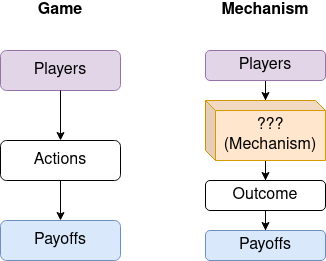
\includegraphics[scale=0.7]{pics/M1/game_vs_mech}
\end{frame}


\begin{frame}{General Problem Set-up}
	In our MD problem, the following environment will be \textbf{fixed}:
	\begin{itemize}
		\item $N$ agents,
		\item set $X$ of \alert{outcomes},
		\item each agent $i$ has \alert{type} $\theta_i\in\Theta_{i}$:
		\begin{itemize}
			\item describes agent's \structure{information},
			\item describes agent's \structure{preferences};
		\end{itemize}
		\item the type profile $\theta=(\theta_1,\dots,\theta_{N})$ is distributed according to a distribution $F$ with p.d.f. $\phi$,
		\begin{itemize}
			\item (often a missing subscript denotes a vector of respective objects)
			\item distribution $F$ is commonly known and agreed upon
		\end{itemize}
		\item each agent has a \alert{utility} function $u_{i}(x,\theta_{i})$ that depends on the collective choice $x \in X$ and his type $\theta_i$,
	\end{itemize}
\end{frame}


\begin{frame}{Social Choice Function}
	\begin{definition}[Social choice function]
		A \alert{social choice function} is a function \alert{$f:\Theta_{1}\times \dots\times\Theta_{N}\rightarrow X$} that assigns to each profile of types $(\theta_{1},\dots,\theta_{N})$ a collective choice $f(\theta_{1},\dots,\theta_{N})\in X$.
	\end{definition}
	\begin{itemize}
		\item gives a desired outcome as a function of the agents' types
	\end{itemize}
\end{frame}


\begin{frame}{Mechanism}
	\begin{itemize}
		\item a mechanism is a game played by the agents
		\item each agent has an action set $A_{i}$ in this game
	\end{itemize}
	\begin{definition}[mechanism]
		A \alert{mechanism} $\Gamma=(A_{1},\dots,A_{N},g(\cdot))$ is a collection of: 
		\begin{itemize}
			\item N \structure{strategy sets} $(A_{1},\dots,A_{N})$ and 
			\item an \structure{outcome function} $g:A_{1}\times\dots\times A_{N}\rightarrow X$.
		\end{itemize}
	\end{definition}
\end{frame}


\begin{frame}{Implementation}
	\begin{definition}[implementation]
		Mechanism $\alert{\Gamma}=(A_{1},\dots,A_{N},g(\cdot))$ \alert{implements} the s.c.f. $\alert{f}$ if there is \structure{an equilibrium} strategy profile $(a_{1}^{*},\dots,a_{N}^{*})$ of the Bayesian game induced by $\Gamma$ \structure{such that} 
		$$\structure{g}(a_{1}^{*}(\theta_{1}),\dots,a_{N}^{*}(\theta_{N})) = \structure{f} (\theta_{1},\dots,\theta_{N})$$ 
		for all $(\theta_{1},\dots,\theta_{N})\in\Theta_{1}\times\dots \times\Theta_{N}$.
	\end{definition}
\end{frame}


\begin{frame}{Summary of definitions}
	\begin{itemize}
		\item S.c.f. $f$ describes what we want to achieve;
		\item Mechanism $\Gamma = (S,g)$ describes what we do and how;
		\item Implementability says whether we have achieved our goal.
	\end{itemize}
\end{frame}


\begin{frame}{Full problem setup}
	\centering
	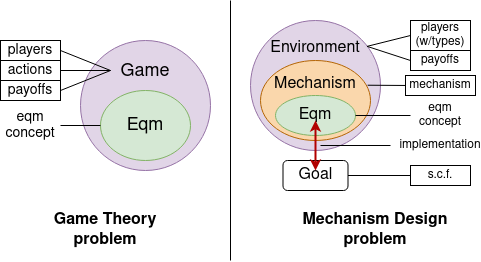
\includegraphics[scale=0.7]{pics/M1/game_vs_mech2}
\end{frame}


\begin{frame}
	(mechanism proposals)
\end{frame}



\section{Revelation Principle}

\begin{frame}{Revelation Principle}
	\begin{itemize}
		\item Main cheat in Mechanism Design! No need to bruteforce through uncountable numbers of different games! It is enough to just... \visible<1>{(\href{https://www.youtube.com/watch?v=dQw4w9WgXcQ}{{click to see more}})}
		\pause
		\item Instead of making players play the game, ask them for their $\theta_i$ and promise to play on their behalf!
		\item Requires that the designer has commitment power.
		\begin{itemize}
			\item Strong assumption, sometimes reasonable(?)
			\item The necessary evil for our purposes.
		\end{itemize}
	\end{itemize}
\end{frame}


\begin{frame}{Revelation Principle: Definitions}
	Fix some s.c.f. $f:\Theta \to X$.
	\begin{definition}[Direct revelation mechanism]
		A \structure{direct revelation mechanism} for $f$ is a mechanism in which $A_i = \Theta_i$ for all $i$ and $g(\theta) = f(\theta)$
	\end{definition}
	
	\begin{definition}[Truthuful implementation]
		S.c.f. $f$ is \structure{truthfully implementable} if it can be implemented by a direct revelation mechanism.
	\end{definition}
\end{frame}


\begin{frame}{Revelation Principle: Statement}
	\begin{block}{Revelation principle (blanket statement)}
		Suppose there exists a mechanism $\Gamma=(A_{1},\dots,A_{N},g)$ that implements the social choice function $f$.\\ Then $f$ is \structure{truthfully implementable}.
	\end{block}
	\medskip
	\begin{itemize}
		\item The statement above is informal.
		\begin{itemize}
			\item ``Implementation'' requires ``an equilibrium'', which can mean a million different things.
		\end{itemize}
		\item We will now focus on specific equilibrium concepts.
	\end{itemize}
\end{frame}
\note{
	\begin{itemize}
		\item We cannot fool agents by designing a very complicated game -- because they are rational and will compute the optimal strategy regardless
		\begin{itemize}
			\item This is, in part, to impose discipline our models -- if can deceive or confuse players then why not just do that.
			\item Economics is the science about being ``technically truthfull'' -- can never lie in equilibrium.
		\end{itemize}
		\item We need a formal equilibrium concept, so let's introduce one...
		\begin{itemize}
			\item Who knows which eqm concepts?
		\end{itemize}
	\end{itemize}
}




\section{Dominant Strategy Implementation}

%TODO 2020: switch from s and S to a and A since there are all actions, not strategies.
\begin{frame}{Recap: Dominant Strategy}
	\begin{itemize}
		\item strategy $a_i$ is a full contingent plan of play
		\item strategy $a_i$ is \alert{dominant} for agent $i$ if it is best \emph{no matter what the other players do}
	\end{itemize}
	\begin{definition}[dominant strategy]
		Given mechanism $\Gamma=(A,g)$,
		$a_{i}: \Theta_{i}\rightarrow A_{i}$ is a \structure{dominant strategy} if for all $\theta_{i}\in \Theta_{i}$
		$$ u_{i}(g(a_{i}(\theta_{i}),a_{-i}),\theta_{i})\geq u_{i}(g(\hat a_{i},a_{-i}),\theta_{i})$$
		for all $\hat a_{i}\in A_{i}$  and all $a_{-i}\in A_{-i}$.
	\end{definition}
	\begin{itemize}
		\item our definition slightly different from the standard -- does not require strict inequality
	\end{itemize}
\end{frame}


\begin{frame}{Dominant Strategy Equilibrium}
	\begin{itemize}
		\item in a \alert{dominant strategy equilibrium} every player plays a dominant strategy
	\end{itemize}
	\begin{definition}[dominant strategy equilibrium]
		A strategy profile $(a_1^*,\dots,a_N^*)$ is a \structure{dominant strategy equilibrium} of mechanism  $\Gamma=(A_{1},\dots,A_{N},g)$ if for all $i$ and all $\theta_{i}\in \Theta_{i}$
		$$ u_{i}(g(a_{i}^{*}(\theta_{i}),a_{-i}),\theta_{i}) \geq u_{i}(g(\hat a_{i},a_{-i}), \theta_{i})$$
		for all $\hat a_{i}\in A_{i}$ and all $a_{-i}\in A_{-i}$.
	\end{definition}

	Now let's finally be formal about all our definitions.
\end{frame}


\begin{frame}{Dominant Strategy Implementation}
	\begin{itemize}
		\item A mechanism \alert{implements $f$ in dominant strategies} if
		\begin{itemize}
			\item the game induced by the mechanism has a dominant strategy equilibrium
			\item the outcome in this equilibrium coincides with $f$
		\end{itemize}
	\end{itemize}
	\begin{definition}[implementation in dominant strategies]
		A mechanism $\Gamma=(A_{1},\dots,A_{N},g)$ \structure{implements} the social choice function $f$ \structure{in dominant strategies} if there exists a dominant strategy equilibrium $(a_1^*,\dots,a_N^*)$ of $\Gamma$ such that $g(a_1^*(\theta_{1}),\dots,a_N^*(\theta_{N}))=f(\theta)$ for all $\theta\in\Theta$.
	\end{definition}
\end{frame}


\begin{frame}{Good Implementation Concept?}
	\begin{itemize}
		\item very robust equilibrium concept
		\begin{itemize}
			\item no need to predict what the other players will play
			\item no need to know the type distribution $\phi$
			\item works even if
			\begin{itemize}
				\item players don't know $\phi$ or even if players believe in different $\phi_{i}$ (protects from players' model misspecification)
				\item players think that other players are not rational
			\end{itemize}
		\end{itemize}
		\item not a panacea
		\begin{itemize}
			\item does not rule out other weird Nash Equilibria (remember SPA)
			\item is not necessarily collusion-proof
			\item does not protect from designer's model misspecification
		\end{itemize}
	\end{itemize}
	Bottom line: it's as good as they get, but far from perfect.
\end{frame}


\begin{frame}{Dominant Strategy Incentive Compatibility}
	\begin{theorem}[Revelation Principle for Dominant Strategies]
		Suppose there exists a mechanism $\Gamma=(A_{1},\dots,A_{N},g)$ that implements the social choice function $f$ in dominant strategies.\\ Then $f$ is \structure{truthfully implementable} in dominant strategies.
	\end{theorem}
	\medskip
	\begin{definition}[Dominant Strategy Incentive Compatibility]
		``$f$ is \alert{dominant strategy incentive compatible} (DSIC)''\\ 
		means the exact same thing as \\
		``$f$ is \structure{truthfully implementable in dominant strategies}''.
	\end{definition}
\end{frame}


\begin{frame}{DS Revelation Principle: Proof}
	Let $\Gamma$ implement $f$ in dominant strategies, i.e. there is a strategy profile  $(a_1^*,\dots,a_N^*)$ such that $g(a_1^*(\theta_{1}),\dots,a_N^*(\theta_{N}))=f(\theta)$ for all $\theta$, and for all $i$ and  $\theta_{i}\in\Theta_{i}$,
	$$ u_{i}(g(a_{i}^{*}(\theta_{i}),a_{-i}),\theta_{i})\geq u_{i}(g(\hat a_{i},a_{-i}),\theta_{i})$$
	for all $\hat a_{i}\in A_{i}$ and all $a_{-i}\in A_{-i}$. 
	
	Then
	$$ u_{i}(g(a_{i}^{*}(\theta_{i}), a_{-i}^{*}(\theta_{-i})),\theta_{i})\geq u_i (g(a^*_i(\hat{\theta}_i), a_{-i}^{*}(\theta_{-i})), \theta_i)$$
	for all $\hat{\theta}_i \in \Theta_i$, $\theta_{-i} \in \Theta_{-i}$. 
	
	Since $g(a^*(\theta)) = f(\theta)$,
	$$ u_i (f(\theta_i,\hat{\theta}_{-i}),\theta_i) \geq u_i (f(\hat{\theta}_i,\hat{\theta}_{-i}), \theta_i)$$
	for all $\hat{\theta}_{-i} \in \Theta_{-i}$.
\end{frame}
\note{
	Main idea: we have IC constraints for the original mechanism. Want to show that IC constraints for a DRM will also hold.
}


\begin{frame}{Revelation Principle: Is it cool or is it cool?}
	\begin{itemize}
		\item Allows to quickly check whether a given $f$ is [DS] implementable.
		\item If yes, gives you a mechanism to implement it.
		\item If not, helps you describe a set of implementable s.c.f. and pick second best.
		\item \emph{Yours today for \soutred{only \$49.99+shipping} FREE with a qualifying Mechanism Design course!}
	\end{itemize}
\end{frame}


\begin{frame}{DSIC: Example}
\begin{example}[Communism]
	\begin{itemize}
		\item society of $N$ people;
		\item each person's productivity either high $\theta^h$ or low $\theta^l$, equal shares of society;
		\item a $\theta^{h}$ ($\theta^{l}$) type produces 4 (2) units per full day
		\item working full day costs 1 unit to the person
		\item working half day costs 0.5 units
		\item the government can only observe the income=production but not the type (nor number of hours worked)
		\item the government can use taxation to redistribute income
		\item Can the government achieve an equal society in which everyone works full time and has an income of 3?
	\end{itemize}
\end{example}
\end{frame}

%TODO: move this to ``arbitrary scf''
%\begin{frame}{DSIC: Weak Preference Reversal Property}
%\begin{itemize}
%	\item ``To each their own'': different types should get their most preferred option among the available ones:
%	$$ u_{i}(f(\theta_{i}', \theta_{-i}), \theta_{i}') \geq u_{i}(f(\theta_{i}'', \theta_{-i}), \theta_{i}')$$
%	$$ u_{i}(f(\theta_{i}', \theta_{-i}), \theta_{i}'') \leq u_{i}(f(\theta_{i}'', \theta_{-i}), \theta_{i}'')$$
%	\item $i$'s preference between $f(\theta_{i}', \theta_{-i})$ and $f(\theta_{i}'', \theta_{-i})$ should flip when his type changes from $\theta_i'$ to $\theta_i''$.
%	\item Obviously a necessary condition for DSIC. Can show it's also sufficient, meaning in the end Preference Reversal is equivalent to $f$ being DSIC.
%\end{itemize}
%\end{frame}



\section{Efficient quasilinear mechanisms: VCG}

\begin{frame}{Quasilinear Preferences}
\begin{itemize}
	\item Instead of allowing all possible preferences, adopt a special structure.
	\item Instead of $x \in X$ describing everything related to outcome, split it into:
	\begin{itemize}
		\item $\alert{k(\theta) \in K}$, ``real/material outcome'' a.k.a. \structure{allocation}
		\item $\alert{t(\theta) \in \mathbb{R}^N}$, \structure{transfers/payments}
	\end{itemize}
	\item Instead of arbitrary $u_i(x,\theta)$ focus on \structure{quasilinear preferences}:
	$$\alert{ u_i(x,\theta_i) = v_i(k,\theta_i) - t_i }$$
	\vspace{-1em}
	\item S.c.f. is $f(\theta) = \left( k(\theta), t_1(\theta), ..., t_N(\theta) \right)$
\end{itemize}
\end{frame}
\note{
	Everything before was very abstract. Let's get to particulars and implement efficient scf. To make things easier, focus on quasilinear setting (allow numeraire=money=transferable utility).
}


\begin{frame}{Quasilinear Preferences}
\begin{itemize}
	\item Restrictions include:
	\begin{itemize}
		\item Monetary transfers always available,
		\item utility is linear in money,
		\item marginal utility of money is constant across types and people.
	\end{itemize}
	\item All three are sometimes restrictive, the latter two especially. But let's roll with it.
\end{itemize}
\end{frame}


\begin{frame}{Efficient Implementation}
\begin{itemize}
	\item A frequent question: ``Dr.Professor, how can we as society implement \structure{the efficient outcome}?''
	\item Reminder: efficient outcome $x^*(\theta) = (k^*(\theta),t^*(\theta))$ is 
	\vspace{-0.5em}\begin{align*}
	x^*(\theta) &= \arg \max_x \sum_{i=1}^N u_i(x,\theta_i) \\
	&= \arg \max_{(k,t)} \sum_{i=1}^N \left[v_i(k,\theta_i) - t_i\right]
	\end{align*}
	\item Transfers just reallocate utility across agents, so focus on \structure{efficient allocation $k^*(\theta)$}:
	\vspace{-1em}\begin{align*}
	k^*(\theta) = \arg \max_k \sum_{i=1}^N v_i(k,\theta)
	\end{align*}
\end{itemize}
\end{frame}


\begin{frame}{Efficient Implementation}
\begin{itemize}
	\item What we as designers want:
	\vspace{-1em}\begin{align*}
	\max \sum_{i=1}^N v_i(k,\theta_i)
	\end{align*}
	\item What agent $i$ wants:
	\vspace{-1em}\begin{align*}
	\max v_i(k,\theta_i) - t_i
	\end{align*}
	\item How to reconcile the two?
\end{itemize}
\end{frame}


\begin{frame}{VCG Mechanism: Groves' Transfers}
\begin{itemize}
	\item More formally, the problem of agent $i$ of type $\theta_i$ is:
	\vspace{-0.5em}\begin{align*}
	\max_{\hat{\theta}_i} \left\{  v_i(k^*(\hat{\theta}_i,\theta_{-i}),\theta_i) - t_i(\hat{\theta}_i,\theta_{-i}) \right\}
	\end{align*}\vspace{-1em}
	\item Try \alert<1>{Groves' transfers}:
	\vspace{-0.5em}\begin{align*}
	\structure<1>{ t_{i}(\theta)=-\left(\sum_{j\neq i} v_{j}(k^*(\theta_i, \theta_{-i}), \theta_{j}) \right) + h_{i}(\theta_{-i}) }
	\end{align*}\vspace{-1em}
	\item Agent's problem is now
	\vspace{-0.5em}\begin{align*}
	\max_{\hat{\theta}_i} \left\{ \structure{v_i(k^*(\alert<3>{\hat{\theta}_i},\theta_{-i}),\theta_i) + \left( \sum_{j\neq i} v_{j}(k^*(\alert<3>{\hat{\theta}_i},\theta_{-i}), \theta_{j}) \right)} - h_{i}(\theta_{-i}) \right\}
	\end{align*}
\end{itemize}
\end{frame}
\note{
	Note on interpretation: the happier you make others, the less you have to pay
}


\begin{frame}{VCG Mechanism: Groves' Transfers}
\begin{itemize}
	\item Agent's problem is now
	\vspace{-0.5em}\begin{align*}
	\max_{\hat{\theta}_i} \left\{ \structure{ \sum_{j=1}^N v_{j}(k^*(\alert{\hat{\theta}_i},\theta_{-i}), \theta_{j}) } - h_{i}(\theta_{-i}) \right\}
	\end{align*}
	\item Every agent $i$ maximizes welfare!
	\begin{itemize}
		\item Optimal to report true $\hat{\theta}$,
		\item for any $\theta_{-i}$.
	\end{itemize}
	\item Crucial that $h_i(\theta_{-i})$ does not depend on $i$'s report.
\end{itemize}
\end{frame}
%TODO: VCG proof?


\begin{frame}{VCG Mechanism: Example}
\begin{exampleblock}{Back to Moon Base}
	\begin{itemize}
		\item $N$ citizens decide whether to build a Moon base which costs $c$
		\item citizen $i$ has private valuation $\theta_{i}$ for the base and quasilinear utility
		
		(so if base built then $v_i = \theta_i$, otherwise $v_i = 0$)
	\end{itemize}
\end{exampleblock}
\begin{itemize}
	\item What are Groves' transfers? (Take $h_i(\theta_{-i}) \equiv 0$.)
	% $$ t_i(\theta) = - \mathbb{I} \left\{\sum_{j=1}^N \theta_j \geq c \right\} \cdot \sum_{j \neq i} \theta_j $$
	\item The incentives are there... but at what cost?
\end{itemize}
\end{frame}


\begin{frame}{VCG Mechanism: Clarke Term}
\begin{itemize}
	\item A suggestion for $h_i(\theta_{-i})$ made by Clarke (``pivot mechanism''):
	\vspace{-0.5em}\begin{align*}
	&h_{i}(\theta_{-i})=\sum_{j\neq i} v_{j}(k^*(\theta_{-i}),\theta_{j}),
	\\ &\text{where } k^*(\theta_{-i}) = \arg\max_{k} \sum_{j\neq i}v_{j}(k,\theta_{j}).
	\end{align*}
	\item Resulting \alert{VCG transfers}:
	\vspace{-0.5em}\begin{align*}
	\structure{ t_{i}^{VCG}(\theta) } = -\left(\sum_{j\neq i} v_{j}(k^*(\theta_i, \theta_{-i}), \theta_{j}) \right) + \sum_{j\neq i} v_{j}(k^*(\theta_{-i}), \theta_{j})
	\end{align*}
\end{itemize}
\end{frame}
\note{
	\begin{itemize}
		\item If you ``say nothing'', presumably some outcome is still implemented.
		\item So if you decide to ``say anything'', it is to tilt the decision in your direction at the expense of everyone else.
		\item So you must pay exactly the externality you impose on everyone else.
	\end{itemize}
}


\begin{frame}{VCG Mechanism: Final Transfers}
\begin{align*}
\structure{ t_{i}^{VCG}(\theta) } = -\left(\sum_{j\neq i} v_{j}(k^*(\theta_i, \theta_{-i}), \theta_{j}) \right) + \sum_{j\neq i} v_{j}(k^*(\theta_{-i}), \theta_{j})
\end{align*}
\begin{itemize}
	\item What's the big idea?
	\item Agent $i$ receives the externality his report imposes on others (mind the signs).
	\item $i$'s transfer is non-zero only if his presence affects the decision $k$.
	\item Note that $i$ cannot misreport $\theta_i$ and get lower transfer without also changing $k$.
	\item What are VCG transfers in the Moon Base question?
\end{itemize}
\end{frame}


\begin{frame}{VCG Mechanism: Example}
\begin{example}[Auction]
	\begin{itemize}
		\item One indivisible item to be allocated among $N$ bidders.
		\item Bidder $i$'s valuation is \structure{$\theta_i$} (private info).
		%\item Want to allocate the item efficiently (to whoever values it most).
		\item What is the VCG mechanism?
	\end{itemize}
\end{example}
\begin{itemize}
	\item VCG mechanism is the second-price auction (efficient and DSIC).
	\item Also known as the Vickrey auction (the V in VCG).
\end{itemize}
\end{frame}


\begin{frame}{VCG aftermath}
\begin{itemize}
	\item We have an easy recipe to implement the \structure{efficient} outcome in \structure{dominant} strategies.
	\item Note $k^*$ may account the designer's ($i=0$) utility over outcomes. %TODO: move it somewhere else?
	\item Any problems?
\end{itemize}
\end{frame}
\note{
	\begin{itemize}
		\item It may not be budget balanced or, more generally, maximize revenue...
		\item All DSE issues apply (collusion, misspecification, (complexity))
	\end{itemize}
}


\section{Individual Rationality and Budget Balance}

\begin{frame}{Feature example: bilateral trade}
\begin{example}[Bilateral Trade]
	\begin{itemize}
		\item One indivisible good.
		\item Two agents: buyer and seller. 
		\item Private valuations $\theta_b,\theta_s \in [0,1]$ resp.
		\item Find the VCG transfers (take no trade as efficient when $\theta_s = \theta_b$).
	\end{itemize}
\end{example}
\end{frame}


\begin{frame}{Feature example: bilateral trade}
\begin{itemize}
	\item If you did everything correctly, you'll get
	\begin{align*}
		t_b^{VCG}(\theta) &= \theta_s \cdot \mathbb{I} \{ \theta_s < \theta_b \} 
		\\ t_s^{VCG}(\theta) &= \theta_b \cdot \mathbb{I} \{ \theta_s \geq \theta_b \} 
	\end{align*}
	\pause
	\item The seller pays to keep the good and doesn't get anything from selling it. Good deal?
\end{itemize}
\end{frame}


\begin{frame}{Individual rationality}
\begin{itemize}
	\item In many settings can't force players to participate in mechanism:
	\begin{definition}[IR]
		A mechanism $\Gamma$ is:
		\begin{itemize}
			\item \structure{interim} \alert{individually rational} if
			$\mathbb{E}_{\theta_{-i}} \left[u_i(\theta_i,\theta_{-i})\right] \geq 0$ for all $\theta_i$;
			\item \structure{ex post} \alert{individually rational} if
			$u_i(\theta_i,\theta_{-i}) \geq 0$ for all $\theta$.
		\end{itemize}
		
		
	\end{definition}
	\item (substitute $0$ by $i$'s outside option if non-zero)
	\item expectation means that distribution of $\theta$s now matters!
\end{itemize}
\end{frame}


\begin{frame}{Detour -- brief review}
\begin{itemize}
	\item \structure{ex ante} = $i$ knows nothing;
	\item \structure{ex interim} = $i$ knows $\theta_i$;
	\item \structure{ex post} = $i$ knows $\theta_i$ and $\theta_{-i}$.
	\item We'll mostly work with interim IR; 
	\item ex post IR is also sometimes used in the literature.
\end{itemize}
\end{frame}


\begin{frame}{Budget balance}
\begin{itemize}
	\item VCG for bilateral trade example is not IR for seller (outside option = keep the good).
	\pause\medskip
	\item If we want mechanism to be IR, easy solution is to decrease $t_i(\theta)$ by a million $\forall \theta$.
	\item But that's expensive -- want mechanism to be \structure{budget balanced}:
	\pause
	\begin{definition}[BB]
		\begin{itemize}
			\item Mechanism $\Gamma$ is \structure{ex ante} \alert{budget balanced} if $\mathbb{E}_\theta \left[ \sum_{i=1}^N t_i (\theta) \right] \geq 0$;
			\item Mechanism $\Gamma$ is \structure{ex post} \alert{budget balanced} if $\sum_{i=1}^N t_i (\theta) \geq 0$ for all $\theta$.
		\end{itemize}
	\end{definition}
	\item Mechanism is \structure{exactly BB} if the above hold with equalities.
	\item If $\Gamma$ is ex post BB then it is ex ante BB (prove).
\end{itemize}
\end{frame}


\begin{frame}{IR vs BB}
\begin{itemize}
	\item Fundamental tension between IR and BB.
	\item Back to bilateral trade example: does there exist a mechanism that is
	\begin{itemize}
		\item efficient,
		\item DSIC,
		\item IR,
		\item BB?
	\end{itemize}
	\pause
	\item VCG was not IR, but it's just one mechanism. Can we say anything about other mechanisms?
	\begin{itemize}
		\item Not in most general case*, but all examples (trade, auction, pub.project) fit a much narrower model where we can.
		\item *though see Prop 23.C.5 in MWG
	\end{itemize}
\end{itemize}
\end{frame}





\section{Monotonicity and Payoff Equivalence}

%TODO: cut the euclidean stuff out?
\begin{frame}{The Euclidean model}
\begin{itemize}
	\item Make the following assumptions on top of quasilinearity:
	\begin{itemize}
		\item $\theta_i \in \Theta_{i} = [\underline{\theta}_i, \bar{\theta}_i]$, full support;
		\item $k \in K \subseteq \mathbb{R}^N$, $K$ compact, convex set;
		\item $u_i(x,\theta_i) = \theta_i k_i - t_i$.
	\end{itemize}
	\item I'll call the above \alert{the Euclidean model} (not standard name).
	\item We'll derive two \structure{necessary} conditions for $\Gamma$ to be \structure{DSIC} in \structure{Euclidean} model.
	\item Given $\Gamma$, denote $U_i(\theta_i, \theta_{-i}) := u_i\left(x(\theta_i, \theta_{-i}), \theta_i \right)$.
\end{itemize}
% Examples of non-Euclidean setting -- multiproduct auction, social choice between multiple alternatives.
\end{frame}


\begin{frame}{Monotonicity}
\begin{itemize}
	\item Assume $\Gamma$ is a \structure{direct} mechanism (or consider its direct equivalent).
	\item Play a bit with $i$'s IC (truthtelling constraint): 
	
	for any $i,\theta_i,\hat{\theta}_i,\theta_{-i}$,
	{ \footnotesize
		\begin{align*}
			U_i(\theta_i, \theta_{-i}) &\geq u_i\left(x(\hat{\theta}_i,\theta_{-i}), \theta_i \right)
			\\ 
			\visible<2->{ &\equiv \theta_i k_i(\hat{\theta}_i,\theta_{-i}) - t_i (\hat{\theta}_i,\theta_{-i})}
			\\ 
			\visible<3->{&= \hat{\theta}_i k_i(\hat{\theta}_i,\theta_{-i}) - t_i (\hat{\theta}_i,\theta_{-i}) + \left(\theta_i - \hat{\theta}_i \right) k_i(\hat{\theta}_i,\theta_{-i})}
			\\ 
			\visible<4->{&= U_i(\hat{\theta}_i, \theta_{-i}) + \left(\theta_i - \hat{\theta}_i \right) k_i(\hat{\theta}_i,\theta_{-i})}
		\end{align*}
	}
\end{itemize}
\end{frame}


\begin{frame}{Monotonicity}
\begin{itemize}
	\item In the end:
	\vspace{-0.5em}\begin{align*}
		U_i(\theta_i, \theta_{-i}) &\geq U_i(\hat{\theta}_i, \theta_{-i}) + \left(\theta_i - \hat{\theta}_i \right) k_i(\hat{\theta}_i,\theta_{-i}).
	\end{align*}\vspace{-1em}
	\item Similarly, type $\hat{\theta}_i$ should not want to report $\theta_i$:
	\vspace{-0.5em}\begin{align*}
		U_i(\hat{\theta}_i, \theta_{-i}) &\geq U_i(\theta_i, \theta_{-i}) + \left(\hat{\theta}_i - \theta_i \right) k_i(\theta_i,\theta_{-i}).
	\end{align*}\vspace{-1em}
	\pause
	\item Combining the two \structure<3->{for $\theta_i > \hat{\theta}_i$}, we get
	{\small \vspace{-0.5em}\begin{align*}
			k_i(\theta_i,\theta_{-i}) 
			\geq 
			\frac{ U_i(\theta_i, \theta_{-i}) - U_i(\hat{\theta}_i, \theta_{-i}) }{ \theta_i - \hat{\theta}_i } 
			\geq 
			k_i(\hat{\theta}_i,\theta_{-i}),
		\end{align*}\vspace{-1em}}
	\pause
	\item meaning \structure{$k_i(\theta_i,\theta_{-i}) \geq k_i(\hat{\theta}_i,\theta_{-i})$} -- allocation must be \alert{monotone}.
	\item DSIC: ``Those who value things more should get more things.''
\end{itemize}
\end{frame}


\begin{frame}{Monotonicity}
\structure{Monotonicity}:
\begin{itemize}
	\item is necessary for $f$ to be DSIC in Euclidean settings
	\item is related to ``weak preference reversal property'' we saw for general mechanisms.
	\item has versions for settings more general than Euclidean and less general than quasilinear (B{\"o}rgers 5.3-5.7).
	\begin{itemize}
		\item $\Theta_i$ being one-dimensional is the most important assumption in getting such conditions.
	\end{itemize}
\end{itemize}
From \structure{monotonicity} we can build up to \structure{payoff equivalence}, 

the second cool result in mechanism design (after revelation principle, not monotonicity).
\end{frame}


\begin{frame}{Payoff Equivalence}
\begin{itemize}
	\item $k_i(\theta_i,\theta_{-i})$ is monotone in $\theta_i$, hence continuous a.e.: $\lim_{\hat{\theta}_i \to \theta_i} k_i(\hat{\theta}_i,\theta_{-i}) = k_i(\theta_i,\theta_{-i})$.
	\pause
	\item Together with the big inequality 
	{\begin{align*}
			k_i(\theta_i,\theta_{-i})
			\geq 
			\frac{ U_i(\theta_i, \theta_{-i}) - U_i(\hat{\theta}_i, \theta_{-i}) }{ \theta_i - \hat{\theta}_i } 
			\geq 
			k_i(\hat{\theta}_i,\theta_{-i}),
	\end{align*}}
	
	this means that a.e.
	\pause
	\begin{align*}
		\frac{\partial U_i(\theta_i,\theta_{-i})}{\partial \theta_i} = \lim_{\hat{\theta}_i \to \theta_i} \frac{ U_i(\theta_i, \theta_{-i}) - U_i(\hat{\theta}_i, \theta_{-i}) }{ \theta_i - \hat{\theta}_i }  = k_i(\theta_i,\theta_{-i}).
	\end{align*}
\end{itemize}
\end{frame}


\begin{frame}{Payoff Equivalence}
\begin{itemize}
	\item So if $k(\theta)$ is integrable in $\theta_i$ (e.g. if it's bounded) then for all $\theta_i$
	\begin{align*}
		\structure{
			U_i(\theta_i, \theta_{-i}) = U_i (\underline{\theta}_i,\theta_{-i}) + \int_{\underline{\theta}_i}^{\theta_i} k_i(s,\theta_{-i}) d s
		}
	\end{align*}
	\item This is \alert{payoff equivalence} a.k.a. envelope representation of payoffs a.k.a. Mirrlees condition.
\end{itemize}
\end{frame}


\begin{frame}{Payoff Equivalence}
\begin{theorem}[Payoff Equivalence for DSIC mechanisms]
	For any two DSIC DRMs with $x = (k,t)$ and $x' = (k',t')$ respectively, 	
	\structure{if $k(\theta)=k'(\theta)$} for all $\theta$ \alert{then $t_i(\theta) = t'_i(\theta) + c_i (\theta_{-i})$} for all $\theta$ for some $c_i(\theta_{-i})$.
\end{theorem}
\pause
\begin{itemize} 
	\item Given allocation $k$ (doesn't have to be efficient), utility of one type (usually ``lowest'' type) pins down utils of all types of player $i$ given fixed $\theta_{-i}$.
	\pause
	\item Equivalently, have only one degree of freedom for $i$'s transfers given $\theta_{-i}$.
	\item Remind anything?
\end{itemize}
\end{frame}


\begin{frame}{Payoff Equivalence of Efficient Mechanisms}
\begin{itemize}
	\item Recall Groves' transfers: efficient $k^*$ can be impl-d in DS by
	\vspace{-0.5em}\begin{align*}
		t_{i}(\theta) &= -\left(\sum_{j\neq i} v_{j}(k^*(\theta_i, \theta_{-i}), \theta_{j}) \right) + h_{i}(\theta_{-i})
		\\ &= \structure{-\left(\sum_{j\neq i} \theta_j k_j^*(\theta_i, \theta_{-i}) \right)} + h_{i}(\theta_{-i})
	\end{align*}
	
	\structure<1>{for some $h_i(\theta_{-i})$.}
	\pause
	\item Payoff equivalence implies that \alert{efficient} $k^*$ in a \alert{Euclidean} model can \alert{ONLY} be implemented by some \structure{Groves'} mechanism.
	% Similarity is that there's just one DoF for i's payoffs
\end{itemize}
\end{frame}


\begin{frame}{Back to bilateral trade}
\begin{itemize}
	\item Remember how this detour started?
\end{itemize}
\begin{example}[Bilateral Trade]
	\begin{itemize}
		\item One indivisible good.
		\item Two agents: buyer and seller. 
		\item Private valuations $\theta_b,\theta_s \in [0,1]$ resp.
		\item Is there an \structure{efficient, DSIC, ex post IR, ex post BB} mechanism?
	\end{itemize}
\end{example}
%do on the board
\end{frame}





\section{Bayesian Implementation}

\begin{frame}{DSIC vs BIC}
\begin{itemize}
	\item We've done DS implementation so far. Robust but demanding.
	\item Now: believe that agents are Bayesian, use standard Bayes-Nash Equilibrium as solution concept.
	\pause
	\item Weaker equilibrium concept, so
	\begin{itemize}
		\item less confident it will produce the intended outcome, but
		\item can implement more s.c.f-ns. 
		\item (there's a literature studying whether sets of DSIC and BIC s.c.f-ns are equal in special settings)
	\end{itemize}
	\item Now prior $\phi$ about the distribution of types becomes more relevant (though we already used it when talking about revenue)
\end{itemize}
%TODO: can say a few more words that DSIC is not much more restrictive than BIC, and on the other hand that DSIC is not a guarantee either (e.g. funky eqa in SPA)
\end{frame}


\begin{frame}{Bayesian Implementation}
Start with the general model as before:
\begin{itemize}
	\item $N$ agents;
	\item set of alternatives $X$;
	\item type $\theta_{i}\in\Theta_{i}$ is private information of $i$;
	\item common prior $\phi \in \varDelta(\Theta)$ about distribution of types;
	\item each agent uses Bayes' rule to form a belief over other agents' types\\
	$$\phi(\theta_{-i}|\theta_{i}) = \phi(\theta_{i},\theta_{-i}|\theta_{i}) = \frac{\phi(\theta_{i}, \theta_{-i}) }{\int_{\tilde\theta_{-i}\in\Theta_{-i}} \phi(\theta_{i},\tilde\theta_{-i}) d\tilde{\theta}_{-i}}.$$
\end{itemize}
\end{frame}


\begin{frame}{Bayes-Nash Equilibrium}
\begin{definition}[Bayes-Nash equilibrium]
	The \structure{strategy profile} $s^* =(s_{1}^*,\dots,s_{N}^*)$ with $s_i^*: \Theta_i \to S_i$ is a \alert{Bayesian Nash equilibrium} of the mechanism $\Gamma=(S_{1},\dots,S_{N},g)$ if, for all $i$ and all $\theta_{i}\in\Theta_{i}$,
	$$E_{\theta_{-i}}\left[u_{i}(g(s_i^*(\theta_i),s_{-i}^*(\theta_{-i})),\theta_{i})|\theta_{i}\right]\geq E_{\theta_{-i}}\left[u_{i}(g(\hat s_i,s_{-i}^*(\theta_{-i})),\theta_{i})|\theta_{i}\right]$$
	for all $\hat s_{i}\in S_{i}$.
\end{definition}
\pause
\begin{itemize}
	\item Standard Nash Eqm reasoning: given that everyone else plays eqm strats, $i$ has no incentive to deviate.
	\item (This definition is for pure strategies, but there is no problem in allowing for mixed strategies.)
\end{itemize}
%TODO2020: mention Che-He-Li-Sun (2019) who show that for any stochastic mechanism there is an equivalent deterministic mechanism.
\end{frame}


\begin{frame}{Bayesian Implementation}
\begin{definition}[Bayesian implementation]
	\structure{Mechanism} $\Gamma=(S_{1},\dots,S_{N},g)$ \alert{implements \structure{s.c.f. $f$} in Bayes-Nash equilibrium} if there is a BNE $s^*=(s_{1}^*,\dots,s_{N}^*)$ of $\Gamma$ such that $f(\theta)=g(s^{*}(\theta))$ for all $\theta\in \Theta$.
\end{definition}
\pause
\begin{definition}[Bayesian implementability]
	\structure{S.c.f. $f$} is \alert{implementable in BNE} if there exists $\Gamma$ which implements it in BNE.
\end{definition}
\end{frame}


\begin{frame}{Truthful Bayesian Implementation}
\begin{definition}[Truthful Bayesian implementation]
	\structure{S.c.f. $f$} is \alert{truthfully implementable in BNE} (=Bayesian Incentive Compatible, \alert{BIC}) if $s_{i}^*(\theta_{i})=\theta_{i}$ is a BNE of the direct revelation mechanism $\Gamma=(\Theta_{1},\dots,\Theta_{N},f)$. 
	\bigskip
	
	That is, for all $i,\theta_{i}$, and $\hat{\theta}_{i}\in\Theta_{i}$,
	\vspace{-0.5em}\begin{align*}
		E_{\theta_{-i}}\left[u_{i}(f(\theta_i,\theta_{-i}),\theta_{i})|\theta_{i}\right]\geq E_{\theta_{-i}}\left[u_{i}(f(\hat \theta_{i},\theta_{-i}),\theta_{i})|\theta_{i}\right].
	\end{align*}\vspace{-1em}
\end{definition}
\pause
Every player is asked for their type; reporting truthfully is a BNE.
\end{frame}


\begin{frame}{Revelation principle}
\begin{theorem}[Revelation principle for Bayes-Nash equilibrium]
	\structure{If} there exists a mechanism $\Gamma=(S_{1},\dots,S_{N},g)$ that \structure{implements} $f$ in BNE, 
	\alert{then} $f$ is \alert{truthfully implementable} in BNE.
\end{theorem}
\end{frame}


\begin{frame}{BIC: Efficient Mechanisms}
\begin{itemize}
	\item Skip general settings, focus on \alert{quasilinear} straight away.
	\begin{itemize}
		\item $u_i(\theta) = v(k(\theta),\theta_i) - t_i(\theta)$
	\end{itemize}
	\item Mission same: find mechanism that implements the \structure{efficient} $k^*(\theta)$.
	\pause
	\item We'll look at two:
	\begin{itemize}
		\item \structure{AGV} mechanism (d'Aspremont and Gerard-Varet, 1979);
		\item \structure{generalized VCG} mechanism
	\end{itemize}
\end{itemize}
\end{frame}


\section{AGV}

\begin{frame}{AGV mechanism}
\begin{itemize}
	\item Let 
	\vspace{-0.5em}\begin{align*}
		\tilde{t}_i (\theta_i) := \mathbb{E}_{\theta_{-i}} \left[ \sum_{j \neq i} v_j (k^*(\theta_i,\theta_{-i}), \theta_i) | \theta_i \right]
	\end{align*}
	
	be the ``expected externality'' imposed by $i$ on everyone else.
	\item \structure<1>{AGV transfers} are given by
	\vspace{-0.5em}\begin{align*}
		\structure<1>{t_i^{AGV} (\theta) = \alert<2>{\frac{1}{N-1} \sum_{j \neq i} \tilde{t}_j (\theta_j)} \structure<2>{- \tilde{t}_i (\theta_i)}}.
	\end{align*}\vspace{-1em}
	\pause
	\item \structure{The second term} is the averaged version of Groves' transfer,
	\item \alert{the first term} is $h_i(\theta_{-i})$ which balances the budget.
\end{itemize}
\end{frame}


\begin{frame}{AGV mechanism}
\begin{theorem}
	In a quasilinear model, AGV is:
	\begin{itemize}
		\item efficient (by construction),
		\item exactly ex post BB,
		\item BIC.
	\end{itemize}
\end{theorem}
Not necessarily IR. :(
\end{frame}


\begin{frame}{AGV mechanism. Proof: budget balance.}
\begin{itemize}
	\item Observe that
	\vspace{-0.5em}\begin{align*}
		\sum_i t_i^{AGV} (\theta) = \sum_i \left[ \frac{1}{N-1} \sum_{j \neq i} \tilde{t}_j (\theta_j) - \tilde{t}_i (\theta_i) \right].
	\end{align*}
	\item For any $j$, RHS has:
	\begin{itemize}
		\item $N-1$ terms of the form $\frac{1}{N-1} \tilde{t}_j (\theta_j)$, and
		\item $1$ term of the form $-\tilde{t}_j(\theta_j)$.
	\end{itemize}
	\item These cancel out and exhaust all terms in the sum. Therefore, $\sum_i t_i^{AGV} (\theta) = 0$ for all $\theta$ = ex post exact budget balance.
\end{itemize}
\end{frame}


\begin{frame}{AGV mechanism. Proof: BIC.}
\begin{itemize}
	\item If $i$ reports $\hat{\theta}_i$ then receives utility
	{\footnotesize 
		\vspace{-0.5em}\begin{align*}
			\mathbb{E}_{\theta_{-i}} \left[ v_i(k^*(\hat{\theta}_i, \theta_{-i}), \theta_i) + \sum_{j \neq i} v_j(k^*(\hat{\theta}_i, \theta_{-i}), \theta_j) | \theta_i \right] - \frac{1}{N-1} \sum_{j \neq i} \tilde{t}_j (\theta_j)
		\end{align*}
	}
	\item Last term indep of $\hat{\theta}_i$; 
	
	bracket max-d by $\hat{\theta}_i = \theta_i$ for every $\theta_{-i}$ (since $k^*$ efficient), 
	
	so max-d by $\hat{\theta}_i = \theta_i$ in expectation as well.
	
	\item Reporting truth is a best response to $-i$ reporting truthfully 
	
	$\Rightarrow$ truthful reporting is a BNE of the mechanism. \qed
\end{itemize}
\end{frame}


\section{gVCG}

%TODO2020: move gVCG to DSIC (since it is, in fact, DSIC); leave only AGV in BIC for cases when really need budget balance.
\begin{frame}{Generalized VCG}
\begin{itemize}
	\item Now to another mechanism, gVCG (\href{https://sites.google.com/site/vjkrishna/research}{Krishna and Perry, 2000}).
	\item Earlier we normalized everyone's outside options (util from not participating) to zero.
	\item Now allow for type-dependent outside options $\underline{U}_i (\theta_i)$.
	\pause\medskip
	\item Define \structure{least charitable type} $\bar{\theta}_i$ as
	\begin{align*}
		\bar{\theta}_i \in \arg \min_{\theta_i \in \Theta_i} \mathbb{E}_{\theta_{-i}} \left[ \sum_{j=1}^{N} v_j (k^*(\theta_i,\theta_{-i}),\theta_j) - \underline{U}_i (\theta_i) \right]
	\end{align*}
\end{itemize}
%LCT intuition will become clear later...
\end{frame}


\begin{frame}{Generalized VCG}
GVCG mechanism is a DRM with the efficient allocation $k^*(\theta)$ and payments
\begin{align*}
	t_i^{GVCG} (\theta) =& \sum_{j \neq i} v_j (k^*(\bar{\theta}_i,\theta_{-i}),\theta_j) + v_i (k^*(\bar{\theta}_i,\theta_{-i}),\bar{\theta}_i)
	\\& - \sum_{j \neq i} v_j (k^*(\theta_i,\theta_{-i}),\theta_j) - \underline{U}_i (\bar{\theta}_i)
\end{align*}
\pause
Has the usual Groves' term (the third one); the other three guarantee IR.
\end{frame}


\begin{frame}{Generalized VCG}
\begin{theorem}[gVCG part 1]
	In a \structure{quasilinear} model, gVCG is:
	\begin{itemize}
		\item efficient (by construction),
		\item BIC,
		\item interim IR.
		\item %\visible<0>{maximizes expected revenue among all mechanisms that are BIC, IIR, and implement the efficient $k^*$.}
	\end{itemize}
\end{theorem}
Prove BIC (analogous to AGV).
\end{frame}


\begin{frame}{Generalized VCG. Proof: IIR}
Interim expected utility for $\theta_i$ is
{\small
	\begin{align*}
		\mathbb{E}_{\theta_{-i}} \left[ \sum_{j =1}^N v_j (k^*(\theta),\theta_j) - \left. \sum_{j =1}^N v_j (k^*(\bar{\theta}_i,\theta_{-i}),\theta_j) \right|_{\theta_i = \bar{\theta}_i} | \theta_i \right] + \underline{U}_i (\bar{\theta}_i)
		\visible<2>{
			\geq \underline{U}_i(\theta_i)
		}
	\end{align*}
}
\pause
since
\begin{align*}
	\bar{\theta}_i \in \arg \min_{\theta_i \in \Theta_i} \mathbb{E}_{\theta_{-i}} \left[ \sum_{j=1}^{N} v_j (k^*(\theta_i,\theta_{-i}),\theta_j) - \underline{U}_i (\theta_i) | \theta_i \right]
\end{align*}
% Talk about the meaning of LCT here
\end{frame}


\begin{frame}{IR+BB ?}
\begin{itemize}
	\item So we have two mechanisms that implement the \structure{efficient} $k^*$ in \structure{quasilinear} model:
	\begin{itemize}
		\item AGV: BIC + BB,
		\item gVCG: BIC + IIR.
	\end{itemize}
	\pause
	\item Can we have \structure{EFF + BIC + BB + IR}? 
	\begin{itemize}
		\item At least with weak ex ante BB and interim IR?
		\item At least in a \alert{Euclidean} model?
	\end{itemize}
\end{itemize}
\end{frame}


\section{Optimality of gVCG in the Euclidean world}

\begin{frame}{The Euclidean Model (reminder)}
\begin{itemize}
	\item $\theta_i \in \Theta_{i} = [\underline{\theta}_i, \bar{\theta}_i]$, full support;
	\item $k \in K \subseteq \mathbb{R}^N$, $K$ compact, convex set;
	\item $u_i(x,\theta_i) = \theta_i k_i - t_i$.
\end{itemize}
\end{frame}


\begin{frame}{Payoff Equivalence in BIC}
\begin{theorem}[Payoff Equivalence for BIC mechanisms]
	For any two BIC DRMs with $x = (k,t)$ and $x' = (k',t')$ resp.:
	
	\structure{if \quad $\mathbb{E}_{\theta_{-i}} k_i(\theta_i, \theta_{-i}) = \mathbb{E}_{\theta_{-i}} k_i'(\theta_i, \theta_{-i})$} for all $i,\theta_i$,
	
	\alert{then $\mathbb{E}_{\theta_{-i}} t_i(\theta_i, \theta_{-i}) = \mathbb{E}_{\theta_{-i}} t'_i(\theta_i, \theta_{-i}) + h_i$} for all $i,\theta_i$ for some $h_i$.
\end{theorem}
\begin{itemize}
	\item As before, implies that for given $k$ (any, not just the efficient) we only have one degree of freedom for $t_i(\theta)$,
	\begin{itemize}
		\item now ``just one'' instead of ``just one given $\theta_{-i}$''.
	\end{itemize}
\end{itemize}
\end{frame}


\begin{frame}{Payoff Equivalence in BIC. Proof}
\begin{itemize}
	\item Let 
	\vspace{-0.5em}\begin{align*}
		\bar{U}_i (\hat{\theta}_i,\theta_i) &:= \mathbb{E}_{\theta_{-i}} \left[ u_i \left( x(\hat{\theta}_i, \theta_{-i}), \theta_i \right) | \theta_i \right]
		\\
		&\,\,= \mathbb{E}_{\theta_{-i}} \left[ \theta_i k_i(\hat{\theta}_i, \theta_{-i}) - t_i \left( \hat{\theta}_i, \theta_{-i} \right) | \theta_i \right].
	\end{align*}\vspace{-1em}
	
	(do not confuse with $U_i$ in Euclidean model for DS.)
	\pause
	\item Take full derivative w.r.t $\theta_i$ at $\hat{\theta}_i=\theta_i$:
	\vspace{-0.5em}\begin{align*}
		\frac{d}{d \theta_i} \bar{U}_i (\theta_i,\theta_i) &= \left. \frac{\partial}{\partial \hat{\theta}_i} \bar{U}_i (\hat{\theta}_i,\theta_i) \right|_{\hat{\theta}_i=\theta_i} + \left. \frac{\partial}{\partial \theta_i} \bar{U}_i (\hat{\theta}_i,\theta_i) \right|_{\hat{\theta}_i=\theta_i}
		\\ &= \hspace{1.4cm} 0 \hspace{1.4cm} + \mathbb{E}_{\theta_{-i}} \left[k_i (\theta_i, \theta_{-i}) | \theta_i \right]
	\end{align*}\vspace{-1em}
	
	The first term is zero because truthful report $\hat{\theta}_i = \theta_i$ maximizes $\bar{U}_i (\hat{\theta}_i,\theta_i)$.
\end{itemize}
\end{frame}


\begin{frame}{Payoff Equivalence in BIC. Proof}
\begin{itemize}
	\item Then by the Fundamental Theorem of Calculus
	\begin{align*}
		\bar{U}_i (\theta_i) &= \bar{U}_i (\bar{\theta}_i) + \int_{\bar{\theta}_i}^{\theta_i} \frac{d \bar{U}_i}{d \theta_i}(s,s) d s
		\\&= \bar{U}_i (\bar{\theta}_i) + \int_{\bar{\theta}_i}^{\theta_i} \mathbb{E}_{\theta_{-i}} \left[k_i(s,\theta_{-i}) | \theta_i \right] d s,
	\end{align*}
	meaning that $k$ and $\bar{U}_i (\bar{\theta}_i)$ pin down utilities $\bar{U}_i (\theta_i)$ for all $\theta_i$.
	\medskip
	\item Remark: here we used a different argument to get $\frac{d \bar{U}_i (\theta_i,\theta_{i})}{d \theta_i} = \mathbb{E}_{\theta_{-i}} \left[k(\theta_i,\theta_{-i}) | \theta_i \right]$ compared to DSIC proof. Either argument can be used in both proofs.
\end{itemize}
\end{frame}


\begin{frame}{Generalized VCG}
\begin{theorem}[gVCG, part 2]
	In a \alert{Euclidean} model, gVCG is:
	\begin{itemize}{\color{gray}
			\item efficient (by construction),
			\item BIC,
			\item interim IR;}
		\item maximizes expected revenue among all mechanisms that are BIC, IIR, and implement the efficient $k^*$.
	\end{itemize}
\end{theorem}
If gCVG is not ex ante budget balanced, there does not exist a 

\{EFF + BIC + IIR + ex ante BB\} mechanism (so no ex post BB either).
\end{frame}


\begin{frame}{gVCG. Proof: revenue maximizing in Euclidean}
\begin{itemize}
	\item Given revenue equivalence, just need to show we cannot decrease $h_i$ for any player w/o violating IIR.
	\pause
	\item Decreasing $h_i$ only possible if IR slack for \emph{all} types of $i$.
	\pause
	\item But IR binds for $\bar{\theta}_i$: $\bar{U}_i (\bar{\theta}_i) = \underline{U}_i (\bar{\theta}_i)$ (verify). \qed
\end{itemize}
\end{frame}


\section{Myerson-Satterthwaite Theorem}

\begin{frame}{Application: Bilateral Trade}
\begin{example}[Bilateral Trade (revisited)]
	\begin{itemize}
		\item One indivisible good.
		\item Two agents: buyer and seller. 
		\item Private valuations $\theta_b,\theta_s \sim \text{i.i.d.} U[0,1]$ resp.
		\item Is there an \soutred{efficient, DSIC, ex post IR, ex post BB} (NO)
		\structure{efficient, BIC, interim IR, ex ante BB} mechanism?
	\end{itemize}
\end{example}
\begin{itemize}
	\item How can we approach this?
\end{itemize}
\end{frame}


\begin{frame}{Myerson-Satterthwaite Theorem}
\begin{theorem}[Myerson-Satterthwaite]
	There is no efficient, BIC, interim IR, ex ante BB mechanism in bilateral trade.
\end{theorem}
\begin{proof}
	gVCG is not BB.
	% Do on the board.
\end{proof}
\end{frame}
%TODO: more examples? e.g. public good, discrete types? prob before the Euclidean.

%\begin{frame}{Exercises}
%	(problem set on absalon)
%	\begin{enumerate}
%		\item Design an efficient attendance mechanism for our course.
%		\item Solve a problem on VCG.
%	\end{enumerate}
%\end{frame}


% Now let's talk about whether sum of utilities is a good measure of welfare...

%\section{Social Choice Functions}
%
%
%\begin{frame}{Detour: Social Choice Theory}
%\begin{itemize}
%	\item Sum of utilities is just one measure of welfare -- others are available.
%	\item Further: utilities $u_i$ are nice for exploring intrapersonal trade-offs when making decisions;
%	\item not so good for interpersonal comparisons -- how to measure relative preference intensity?
%	\item What do?
%	\item Social Choice Theory (\& Welfare Economics) deal with aggregating individual preferences into social preference.
%\end{itemize}
%\end{frame}
%
%
%\begin{frame}{Social Choice: Axiomatic Approach}
%\begin{itemize}
%	\item If cardinal utilities bad -- can work with ordinal preference relations $\succsim_i$.
%	\item Can impose axioms on how \structure{individual preferences} $\succsim_i$ should map into \structure{social preference} relation $\succsim$ (and/or corresponding social choice function $f$).
%	\item Possible reasonable axioms:
%\end{itemize}
%\begin{description}
%	\item[(A1)] \structure{Domain}: any collection of individual preferences $\left(\succsim_1, ..., \succsim_N \right)$ can be aggregated into $\succsim$.
%	\item[(A2)] \structure{Unanimity}: if $a \succsim_i b$ for all $i$ then $a \succsim b$.
%	\item[(A3)] \structure{Independence of Irrelevant Alternatives}: if $\succsim_i$ and $\succsim'_i$ rank alternatives $a$ and $b$ the same for all $i$ then so should $\succsim$ and $\succsim'$.
%\end{description}
%\end{frame}
%
%
%\begin{frame}{Social Choice: Axiomatic Approach}
%\begin{block}{Arrow's Theorem}
%	With more than three alternatives, if $\succsim$ satisfies (A1)-(A3) then it is dictatorial, i.e. $\exists i: a \succsim b \Leftrightarrow a \succsim_i b$.
%\end{block}
%\begin{block}{Proof}
%	\href{https://link.springer.com/article/10.1007/s00199-004-0556-7}{Geanakoplos, J. (2005). Three brief proofs of Arrow's impossibility theorem. Economic Theory, 26(1), 211-215.}
%	\vspace{8em}
%\end{block}
%\end{frame}
%
%
%\begin{frame}{Social Choice}
%\begin{itemize}
%	\item See Geanakoplos' paper for [slightly] more details on Arrow's Thm, and MWG ch.21 for more details on Social Choice theory.
%	\item Lesson: aggregating preferences is a difficult problem in itself.
%	\item We won't be dealing with this problem in this class, from now on just take $f$ as given.
%\end{itemize}
%\end{frame}
%
%%TODO 2020: talk about median voter thm with single-peaked preferences here



\end{document}